\documentclass{article}
\setlength\parindent{0pt}
\usepackage{booktabs}
\usepackage{tabularx}
\usepackage{graphicx}
\usepackage{soul}
\usepackage{color}

\title{SE 3XA3: Development Plan\\Title of Project}

\author{Team \#17, Test Icicles
		\\ Andrew Bennett 1319879
		\\ Kyriakos Kyprianou  400025691
		\\ Teodor Tomescu 400038361
}

\date{}



\begin{document}

\begin{table}[hp]
\caption{Revision History} \label{TblRevisionHistory}
\begin{tabularx}{\textwidth}{llX}
\toprule
\textbf{Date} & \textbf{Developer(s)} & \textbf{Change}\\
\midrule
Sept. 29th -- Rev0.1 	& Andrew, Kyriakos, Teodor & first draft \\
Dec. 6th  -- Rev1		& Andrew, Kyriakos, Teodor & modified document to match current project. red text shows modifications.\\

\bottomrule
\end{tabularx}
\end{table}

\newpage

\maketitle
\newpage

\section{Team Meeting Plan}

To stay on track with the project and ensure completion of required topics by a set deadline, our team must meet up once a week for an hour. We want to make sure every member has a clear understanding of what is expected of them so these require mandatory participation by all team members. These meeting will take place every Tuesday from 5 PM to 6 PM on the second floor of the Mills library. In the meeting, we will delegate tasks to each member and ensure that they are fully informed on what will be expected of them. Member roles will be discussed in the Team Member roles section of our development plan however these are not necessarily rigid and can change during the software creation process. \\

\noindent An agenda will be needed during meetings to ensure efficient coordination for the team and to allow feedback from each member. We will draft a template to use as an agenda for each weekly meeting which will include the following topics: Feedback \& Questions, Goals, Homework, Timetable, Meeting Review. In each meeting the project manager will keep track of what goes on in the meetings and ensure that every section of the agenda is appropriately filled out.



\section{Team Communication Plan}


Because not every member of our group owns a cell-phone we are currently using Facebook Chat for general communication on a day to day basis. We created a group with all three members in it and thus far it has been great for us to use as a non-technical means of communicating.\\

\noindent We will be using Unity's built in version control software as well as GIT over the course of this project. This is a great method of keeping track of changes are made to our code over time. It is especially useful since there are three of us all working on one project simultaneously and as we're able to keep a detailed report of every code contribution from each member, there is little that can go wrong on the repository. If ever we need to revert a whole commit we can do so as well. Git makes working on a project with multiple members effortless and it’s why we have decided to use it. 


\section{Team Member Roles}

*Every team member is expected to contribute equally on the Unity build on top of their given role.\\

Andrew Bennett -– Graphics, models, individual game features\\

The graphics and model expert will be responsible for overlooking everything pertaining to the graphics and physical modelling of our pinball game. Since he is the most knowledgeable in Unity game design he will also answer any questions pertaining to Unity.\\

Kyriakos Kyprianou-– Project manager, individual game features\\

The project manager will oversee every meeting to ensure that our agenda is satisfied and note everything down in the template. On top of that, he will also organize any additional meetings the group needs to meet deadlines and clarify concerns. Everything will be then relayed to the remaining group members via the Facebook group chat.\\

Teodor Tomescu -– Overall game manager, individual game features\\

The game manager will supervise the overall cohesiveness of the game and make sure that every member’s contributions are up to par with the initial goals that were outlined. He will make sure that members are on time with their work and judge the correctness of build features.


\section{Git Workflow Plan}


Deliberate and organized use of Git \textcolor{red}{and Unity Version control} features will be integral to our project's success. Our Git work flow will incorporate three major branches, Master, Development, Modelling, as well a number of more specific feature branches. \\

The Master branch will be kept up to date with fully functioning and completed feature sets. It will be our production branch. \\

The Development branch will be used to incorporate finished feature changes. \st{and will be the most up-to-date branch encompassing the project.} \\

The Modelling branch will be used for updating the 3D models used in the game. While 3D modelling and game aesthetics are not the focus of our project, they will be updated over the course of the project. Finished changes made to the models or game visuals will be pushed to the Modelling branch, which will later be integrated into the Development branch. \\

\textcolor{red} {Although Git is instrumental for the success of large-scale software projects, we have found that using Unity's on board version control helped simplify things as we had full Git functionality  integrated in the Unity environment. This especially helps during sprints of rapid development as we can all stay up to date with changes very easily.}
\\

Tagging, Issues, and Milestones will also play an important role in our Git workflow. \\

Tags will be used to label every change made to the Master, Development, and Modelling branches. v1.0, v2.0, v3.0 etc will reflect major progress on the project and will be incremented after each push to the Master branch. Sub-versions (1.1, 1.2, 1.3 etc) will be incremented after each push to the Development and Modelling branches. \\

Issues will be used to keep track of bugs that need to be fixed, and likely will be the responsibility of the developer whose code introduced the bug. \\

Milestones will be used as a way to track feature requests and assign tasks to team members. While each team member is encouraged to work on features they would like to see in the project, Milestones will be used for the core features of the project that need to be included. In addition, Milestone 'due dates' will be used to ensure features are completed on time.\\


\section{Proof of Concept Demonstration Plan}


\subsection{Technologies}

Because our project is a 3D game we have decided to build it using Unity, a third party game engine. Some of the reasons for choosing Unity are as follows:\\

\textbf{1.} Unity is a free software.\\

\textbf{2.} Unity is a professional quality game engine. It has been thoroughly tested and is robust and reliable enough to meet all of our needs, including integration of 3D modelling and code, built in testing, and multiple export formats.\\

\textbf{3.} There are an abundance of resources available to assist us in using Unity. Unity has thorough, clear documentation, and because Unity is such a popular game engine, there are numerous third party guides and tutorials covering all aspects of Unity. 

\subsection{Modules + MVP}

The core modules necessary for our game include: \\

\textbf{1.} A pinball 'playing field' consisting of a solid floor, walls, point-scoring obstacles, and 'bumpers', and containing a 'pinball'. \\

\textbf{2.} Realistic game physics which includes simulated gravity, acceleration of the pinball, and collisions between the playing field and the pinball. \\

\textbf{3.} A scoring system that keeps track of how many points the player has accumulated during the game. \\

\textbf{4.} Game-Ready and Game-Over states. The Game-Ready state should have a menu with 'Start Game'\st{and 'View High Scores' options}\textcolor{red}{and 'Exit Game'.} The Game Over state should display the player's score, and a menu button to return back to the main menu. \\

\textcolor{red}{\textbf{5.} A flipper module to control the flippers and assign sufficient power to their action.}\\

\textcolor{red}{\textbf{6.} A spring module to enable the player to power up and launch the ball into play.}\\

\textcolor{red}{\textbf{7.} A module to return the ball back to its starting position once the current ball hit the bottom of the playing field.}\\


The minimum viable product for our project will include a basic 3D model of the pinball, playing field, and bumpers. Gameplay of the MVP will include a pinball that falls due to the effects of gravity and collides with the playing field obstacles including the bumpers. The bumpers should be functional and responsive to player input. 

\subsection{Risks}

The risks for our project are estimated to be manageable. \\

Basic game elements such as models and physics should be relatively straightforward to implement, however one concern is that the game physics (gravity, collisions, acceleration) could feel unrealistic to players. Menus, game states, and a scoring system are also estimated to be low-risk.\\

Testing is an area that will be of some difficulty. Testing of the game code itself can be done through custom testing suites, where we will manually check for edge cases on every variable and function within the code. 

However, due to the graphical nature of a game, there are a number of bugs that could arise from graphics elements including the 3D models. Fortunately, Unity provides testing tools that will help alleviate this concern. 

Unity itself is very simple to install and provides a lot of useful functionality for game developers. Unity's testing tools will be of great use during this project. Likewise, Unity's convenience exporting tools will allow our game to be extremely portable without needing to rewrite our code to suit different software environments. 


\section{Technology}

The engine that we will be using for our game is Unity 3D. We will use C\# in Unity to create scripts and bring the physical model of the game to life. In order to ensure the desired functionality of our game we will be using Unity’s included test framework called Unity Test Tools. This framework is a package that gives developers all the necessary tools require for creating and executing automated tests inside the Unity editor. Using Unity Test Tools, we will be able to create unit tests and integration tests to ensure our code is up to our standards. \\

To create documentation for all of our C\# scripts we will be using a Unity editor plugin that allows the creation of automatically generated documentation via Doxygen. This plugin is made by a private user however it has great reviews and can be easily installed onto Unity. For more information about the plugin you can visit http://www.jacobpennock.com/Blog/unity-automatic-documentation-generation-an-editor-plugin/.


\section{Coding Style}


In our project a coding style that all team members are familiar with will be implemented. Some elements of this include: \\

\textbf{1.} Brace style will be the java variant of K\&R, with braces on the same line as function and class declarations, as well as control statements. \\

\textbf{2.} Tabs will be used rather than spaces for indentation\\

\textbf{3.} In general, line length should be kept under 80 characters. \\

\textbf{4.} Variable names will be kept sensible and will use camel case rather than snake case or pascal case. 
\newpage

\section{Project Schedule}


\begin{figure}[h]
  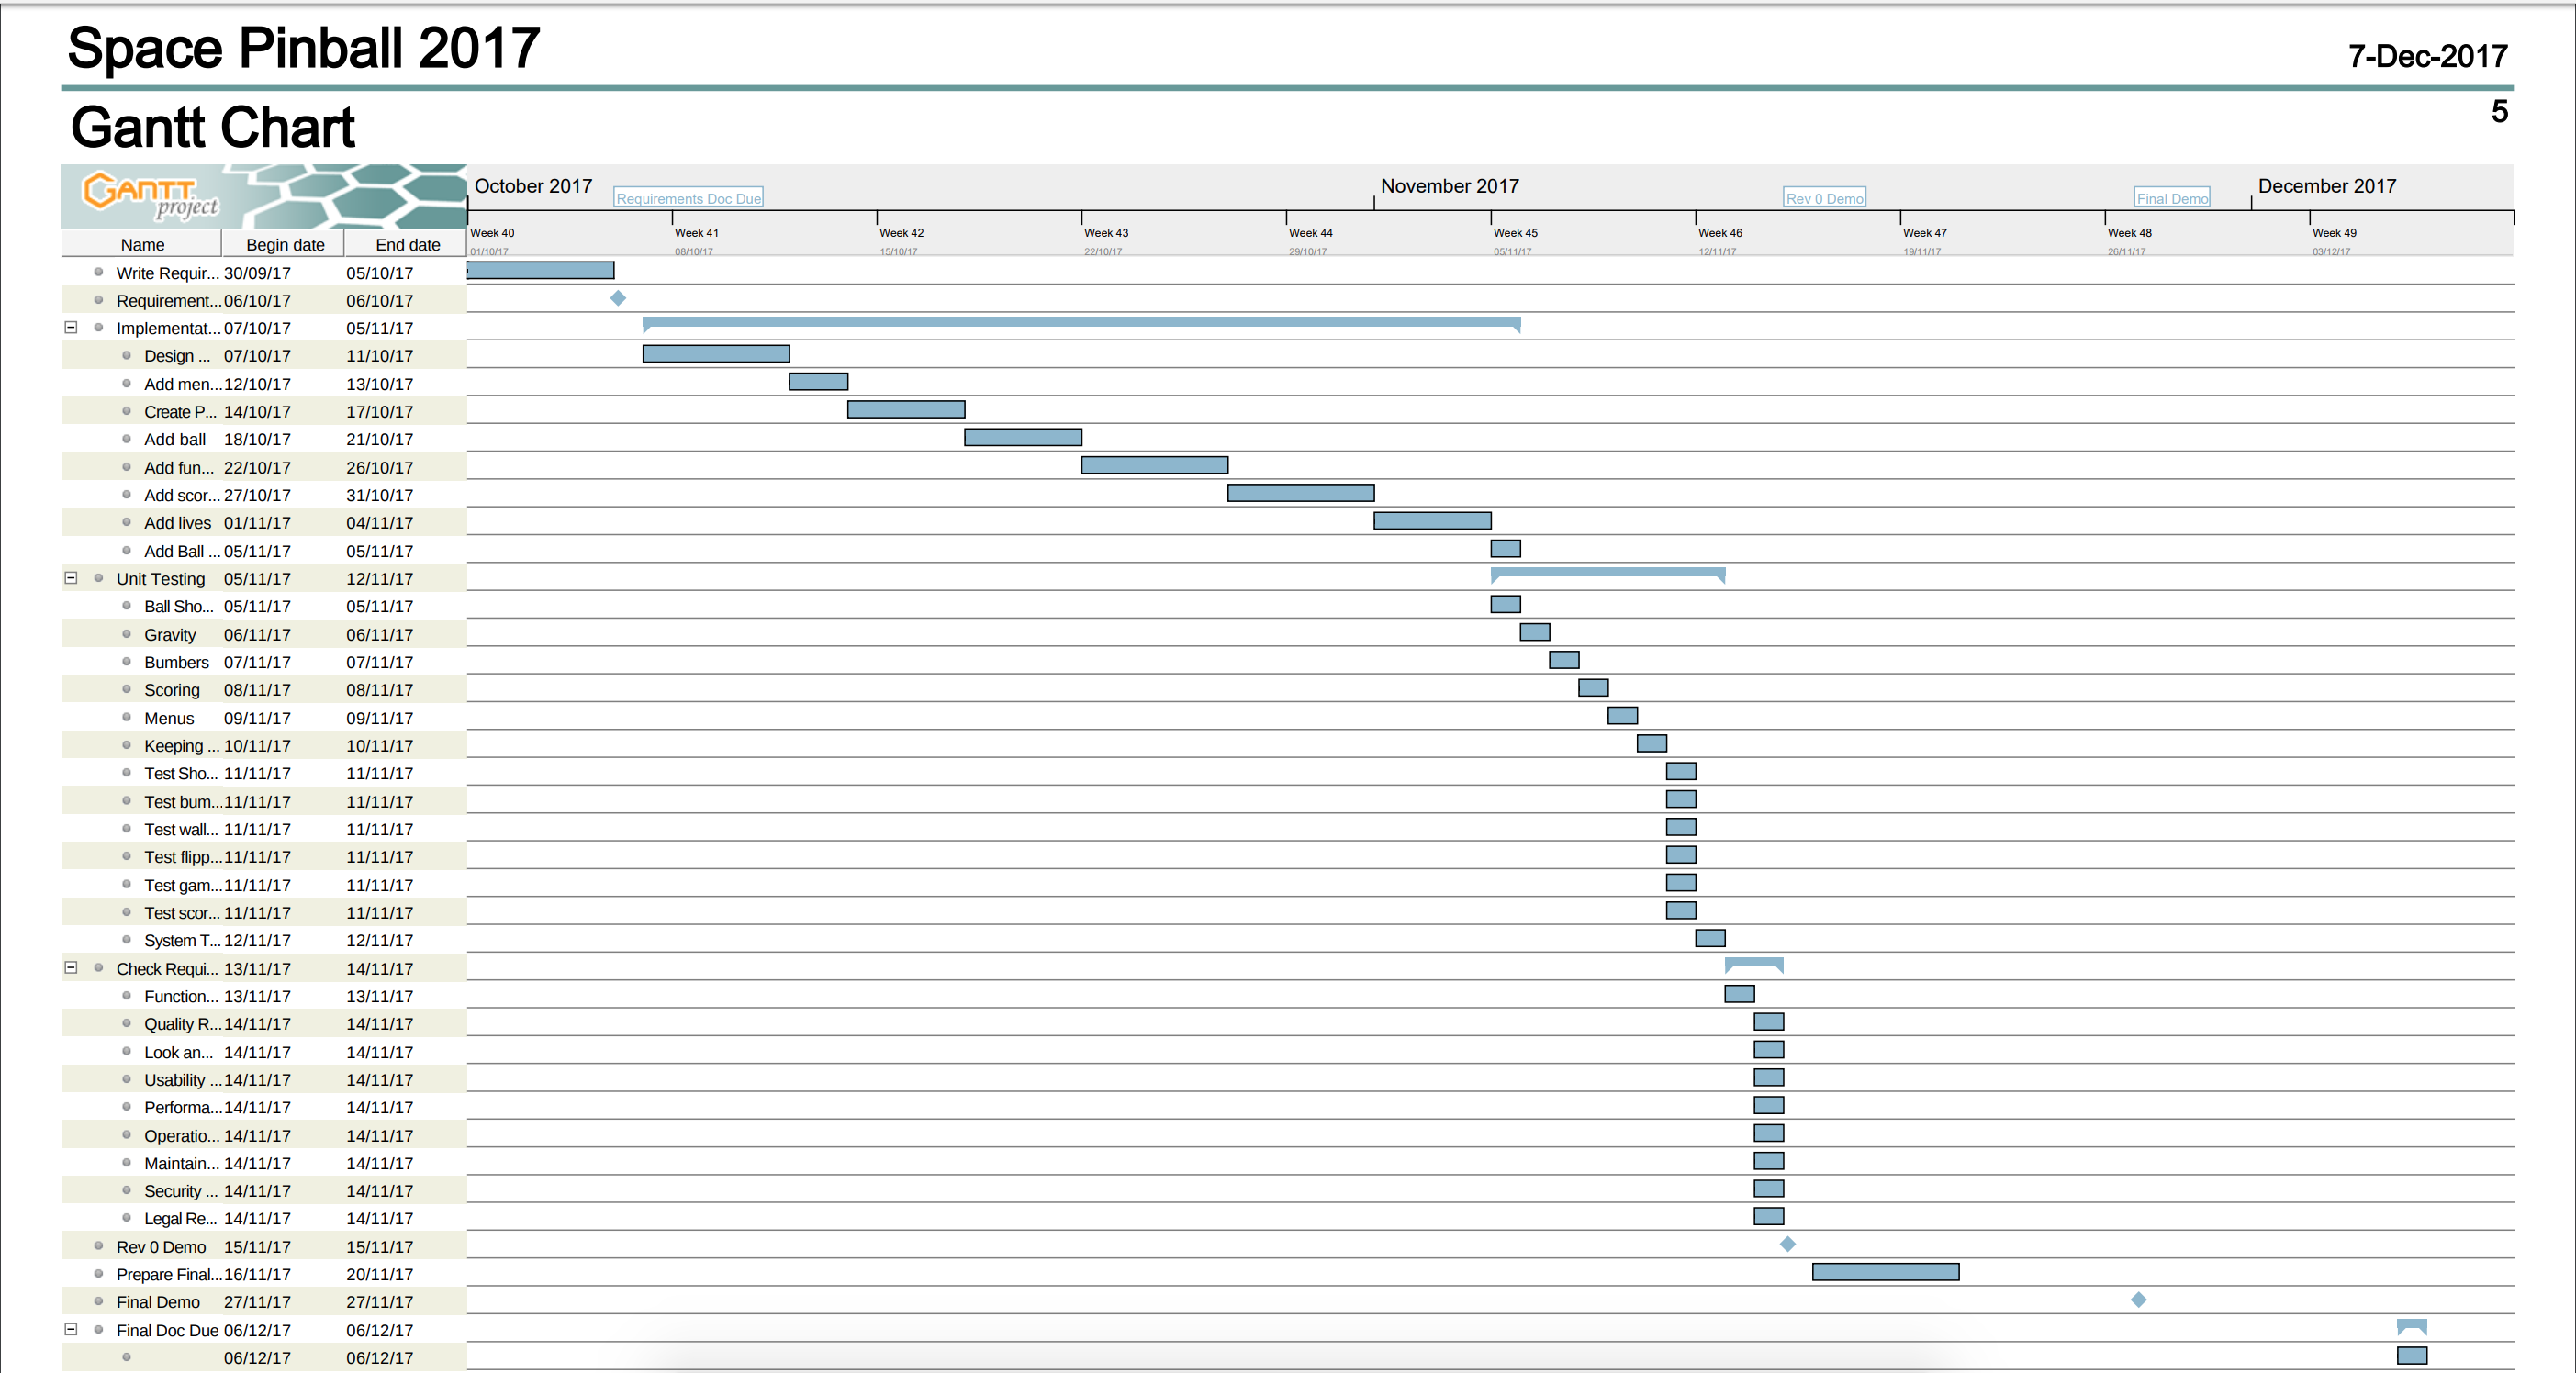
\includegraphics[scale=0.17]{gan.png}
  \caption{Gantt Chart}
  \label{fig:Gantt Chart}
\end{figure}

\begin{figure}[h]
  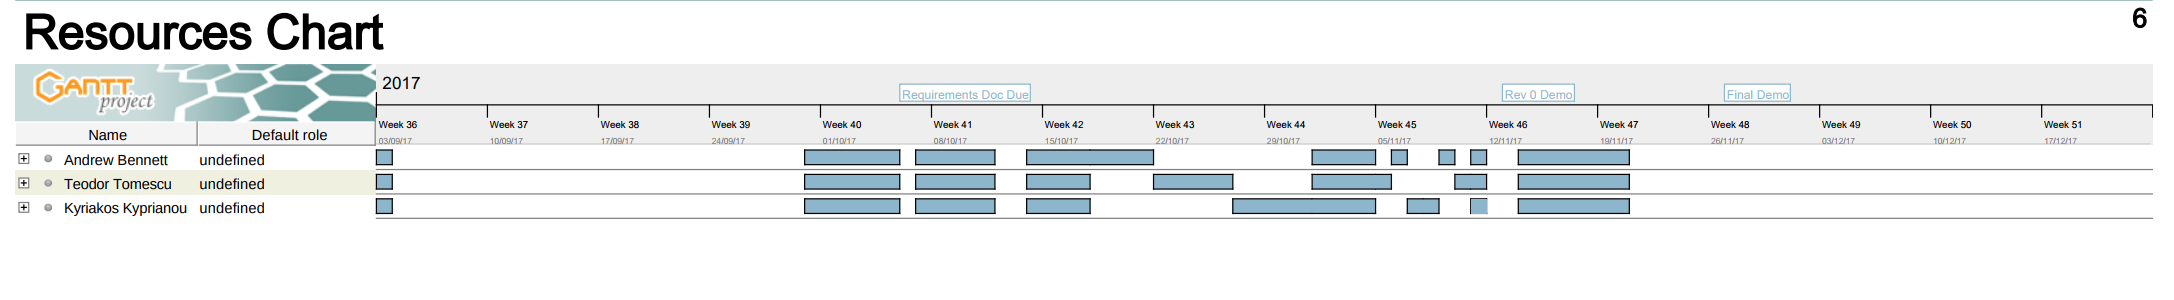
\includegraphics[scale=0.4]{res.png}
  \caption{Resources Chart}
  \label{fig:Resources Chart}
\end{figure}


\section{Project Review}

\end{document}
